\documentclass[a4paper,11pt]{article}
\usepackage[a4paper,top=2cm,bottom=2cm,left=2cm,right=2cm]{geometry}
\usepackage[T1]{fontenc}
\usepackage[utf8]{inputenc}
\usepackage{graphicx}
\usepackage{lmodern}
\usepackage{enumitem}
\usepackage{array}
\usepackage{listings}
\usepackage[italian]{babel}
\usepackage{amsmath}
\usepackage{mathtools}
\usepackage{xspace}
\usepackage{amssymb}
\usepackage[hidelinks]{hyperref}
\usepackage[T1]{fontenc} 
\usepackage{microtype}

\graphicspath{{./Immagini/}} 

\newcommand{\tab}[1]{\hspace{.3\textwidth}\rlap{#1}}
\newcommand{\itab}[1]{\hspace{0em}\rlap{#1}}
\newcommand{\alc}{%                           ALC
   \ensuremath{\mathcal{ALC}}\xspace}
\newcommand{\I}{%                             I (caligraphic)
        \ensuremath{\mathcal{I}}\xspace}
\newcommand{\Q}{%                             Q
  \ensuremath{\mathcal{Q}}\xspace}
\newcommand{\N}{%                             N
  \ensuremath{\mathcal{N}}\xspace}
\newcommand{\Onom}{%                          O
  \ensuremath{\mathcal{O}}\xspace}
\newcommand{\T}{%                             T
  \ensuremath{\mathcal{T}}\xspace}
\newcommand{\A}{%                             T
  \ensuremath{\mathcal{A}}\xspace}
\newcommand{\K}%                              Modal K
        {\ensuremath{\mathbf{K}}\xspace}
\begin{document}

\begin{figure}[!htbp]
	\centering	
	\mbox{%
		\begin{minipage}{.10\textwidth}
			
\includegraphics[scale=0.20]{Immagini/unict.jpg} 
		\end{minipage}%
		\quad
		\begin{minipage}[c]{.60\textwidth}
			\centering
			\Large Universit\`{a} degli Studi di Catania			
			\Large Dipartimento di Matematica e Informatica			
			\Large Corso di Laurea in Informatica triennale			
		\end{minipage}
	}
\end{figure}

\begin{center}
	\hrule
\end{center}

\vspace*{50pt}

\begin{center}
	\LARGE Andrea Costazza
\end{center}

\vspace*{30pt}

\begin{center}
	\LARGE \textbf{Librerie JavaScript per il trattamento di ontologie del Web Semantico con informazioni geolocalizzate}

\end{center}

\vspace*{80pt}

\noindent\hfil\rule{0.2\textwidth}{.4pt}\hfil

\begin{center}
	\Large Relazione progetto finale
\end{center}

\noindent\hfil\rule{0.2\textwidth}{.4pt}\hfil

\vspace*{180pt}

\begin{flushright}
	\Large Relatore

	\Large \textbf {Prof. Domenico Cantone}
\end{flushright}
\begin{flushright}
	\Large Correlatore

	\Large \textbf {Dott. Cristiano Longo}
\end{flushright}
\bigskip
\bigskip

\hrule

\begin{center}
	\Large Anno Accademico 2015/16
\end{center}
\thispagestyle{empty}
\newpage
\null
\thispagestyle{empty}
\newpage

\begin{figure}[!htbp]
\centering	
	\mbox{%
		\begin{minipage}{.10\textwidth}
			
\includegraphics[scale=0.20]{unict.jpg} 
		\end{minipage}%
		\quad
		\begin{minipage}[c]{.60\textwidth}
			\centering
			\Large Universit\`{a} degli Studi di Catania
			
			\Large Dipartimento di Matematica e Informatica
			
			\Large Corso di Laurea in Informatica triennale
			
		\end{minipage}
	}
\end{figure}

\begin{center}
	\hrule
\end{center}

\vspace*{50pt}

\begin{center}
	\LARGE Andrea Costazza
\end{center}

\vspace*{30pt}

\begin{center}
	\LARGE \textbf{Librerie JavaScript per il trattamento di ontologie del Web Semantico con informazioni geolocalizzate}

\end{center}


\vspace*{80pt}

\noindent\hfil\rule{0.2\textwidth}{.4pt}\hfil

\begin{center}
	\Large Relazione progetto finale
\end{center}

\noindent\hfil\rule{0.2\textwidth}{.4pt}\hfil

\vspace*{180pt}

\begin{flushright}
	\Large Relatore

	\Large \textbf {Prof. Domenico Cantone}
\end{flushright}
\begin{flushright}
	\Large Correlatore

	\Large \textbf {Dott. Cristiano Longo}
\end{flushright}

\bigskip
\bigskip

\hrule

\begin{center}
	\Large Anno Accademico 2015/16
\end{center}
\thispagestyle{empty}
\newpage
\null
\thispagestyle{empty}

\newpage

\tableofcontents
\newpage

\section{Introduzione}


\newpage

\section{Web Semantico}
\label{sec:2}
Il termine Web Semantico è un concetto nato solo da pochi anni, dalla mente di Tim Berners-Lee, il quale non solo ha ideato il Word Wide Web(WWW) e il W3C\footnote{\url{http://www.w3.org/}}(World Wide Web Consortium), ma lo ha anche trasformato in qualcosa di rivoluzionario. L'idea di base era quella di associare a tutti i documenti caricati nel web, dei \textbf{metadati}\footnote{Informazione che descrive un insieme di dati. Fonte Wikipedia.} in modo che qualsiasi macchina, motore di ricerca e applicazione fosse in grado di elaborarli con estrema facilità.\newline
Inizialmente si adoperava il semplice \textbf{collegamento ipertestuale,}\footnote{Rinvio da un'unità informativa su supporto digitale ad un'altra. Fonte Wikipedia.} le macchine si limitavano solamente a trasmettere il contenuto, senza possibilità di capire com'era strutturata la pagina.
A tal proposito si utilizza il concetto di \textbf{rappresentazione della conoscenza}.
I sistemi di rappresentazione della conoscenza permettono di usare semantiche formali e simbolismi di carattere matematico, cioè una serie di costrutti sia per definire la sintassi del dominio di interesse, sia una serie di operatori che permettano di dare un significato alle asserzioni.
Con questo ragionamento possiamo quindi costruire una \textbf{base di conoscenza}\footnote{Ambiente volto a facilitare la raccolta, l'organizzazione e la distribuzione della conoscenza. Fonte Wikipedia.}, che permette agli applicativi software e agli agenti automatici di scaricare diverse informazioni che sono relative, per esempio, ad aziende oppure enti culturali e utilizzarle in maniera più adeguata. In questo progetto si utilizza un base di conoscenza realizzata in RDF(vedi Paragrafo \ref{sec:2.1}) ed elaborata attraverso il linguaggio di programmazione Javascript, ma ne parleremo più avanti.\newline
Analizzato i concetti di base del Web Semantico vediamo adesso come è strutturato. Lo si può pensare come un sistema a livelli gerarchico, dove ogni livello è arricchito con nuovi costrutti e simbolismi come mostrato in \textbf{Figura ~\ref{fig:1}}
\begin{figure}[ht]
	\centering
	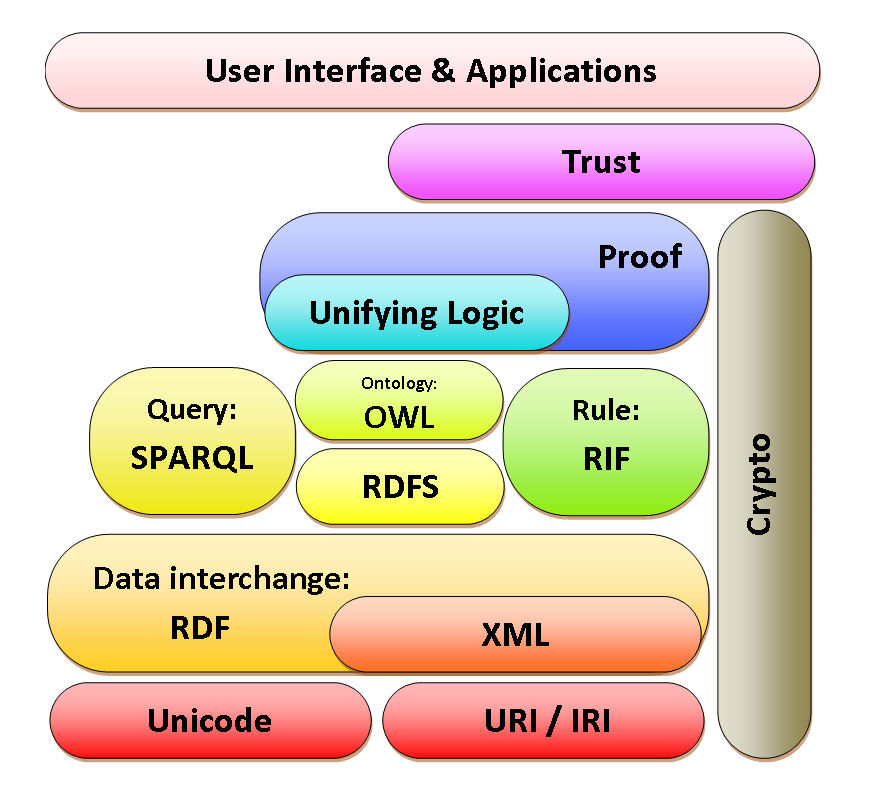
\includegraphics[scale=0.5]{semweb-layers.png}
	\caption{Rappresentazione a livelli del Web Semantico.}
	\label{fig:1}
\end{figure}\newpage I livelli principali\footnote{Tratto da Realizzazione di moduli JAVA per il trattamento del web semantico di Andrea Costazza} sono:
\begin{itemize}	
	\item URI/IRI:\footnote{Uniform Resource Identifier/Internationalized Resource Identifier} Il livello degli indirizzi dove indicano una risorsa generica come ad esempio un pagina web;
	\item Unicode: Standard di codifica dei set di caratteri internazionali. Questo livello permette che tutte le lingue del mondo possano essere utilizzate per qualsiasi pagina web;
	\item XML:\footnote{eXtensible Markup Language} è un linguaggio di markup, simile all'HTML, che è stato progettato per memorizzare e trasportare i dati. Utilizza dei tag che devono rispettare determinate regole e molto spesso fanno uso dei “namespace”, una sorta di vocabolario di termini, a cui si fa riferimento un URI;				
	\item RDF:\footnote{Resource Description Framework} è un linguaggio, proposto dal W3C per rappresentare informazioni sulle risorse attraverso una struttura a grafo. In questo linguaggio le informazioni sono esprimibili con asserzioni (statement) costituite da triple formate da soggetto, predicato e oggetto (identificati come subject, predicate e object, rispettivamente);
	\item RDFS:\footnote{RDF Schema} Estensione di RDF, fornisce elementi di base per la descrizione di ontologie, chiamate vocabolari per le risorse RDF;
	\item OWL:\footnote{Ontology Web Language} è un linguaggio che deriva dalle logiche descrittive, e offre più costrutti rispetto a RDFS. OWL si suddivide in tre categorie: OWL Lite per tassonomie e vincoli semplici, OWL DL per il pieno supporto della logica descrittiva e OWL Full per la massima espressività e la libertà sintattica di RDF;
	\item SPARQL: è un linguaggio di interrogazione per tipologie di dati rappresentati in RDF; è uno degli elementi cardine per sviluppare il web semantico e consente di estrarre informazioni dalle basi di conoscenza distribuite sul web.
\end{itemize}

\subsection{Resource Description Framework (RDF)}
\label{sec:2.1}
Il \textbf{Resource Description Framework(RDF)}, proposto da W3C, è lo strumento base per la realizzazione del Semantic Web. Esso esprime informazioni sulle risorse che possono essere di qualunque tipo, come ad esempio persone o cose.\newline
I dati espressi possono anche essere, ad esempio, informazioni sulle pagine web, contenuti per i motori di ricerca oppure biblioteche elettroniche, sia aziendali che comunali, contenenti moltissime informazioni.
Per descrivere queste informazioni RDF utilizza:
\begin{itemize}
	\item Risorse: come già descritto può essere una qualsiasi cosa;
	\item Proprietà: è una relazione utilizzata per descrivere una risorsa;
	\item Valore: è il valore assunto dalla proprietà; può essere anche una risorsa.
\end{itemize}
Le combinazioni tra Risorse, Proprietà e Valori prendono il nome di \textbf{Asserzioni} (statement), cioè una tripla composta da un soggetto (risorsa), un predicato (proprietà) e un oggetto (valore), come mostrato in \textbf{Figura~\ref{fig:2}}.

\begin{figure}[htbp]
	\centering
	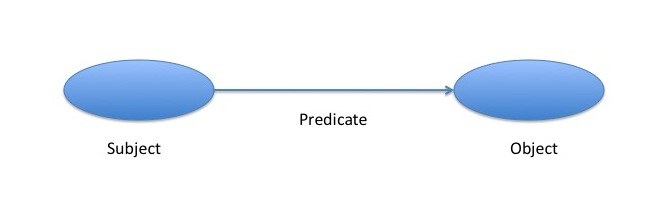
\includegraphics[scale=0.5]{Assertion.jpg}
	\caption{Relazione degli statement.}
	\label{fig:2}
\end{figure}\newpage 

Il soggetto e l'oggetto rappresentano le due risorse, mentre il predicato rappresenta la natura del loro rapporto.\newline Ecco un esempio di triple in RDF:\newline <Napoleone> <è nato> <ad Ajaccio>\newline <Napoleone> <perse> <a Waterloo>.\newline <Jacques-Louis David> <dipinse l'incoronazione> <di Napoleone>.\newline Come si evince dall'esempio Napoleone e soggetto di 2 asserzioni e oggetto dell'altra; questa caratteristica importante, cioè quella di avere la stessa risorsa sia in posizione di soggetto e sia in posizione di oggetto, permette di trovare connessioni tra triple e quindi reperire più informazioni.
Si realizza in questo un grafo dove il soggetto e l'oggetto rappresentano i nodi mentre il predicato corrisponde l'arco.

\begin{figure}[ht]
	\centering
	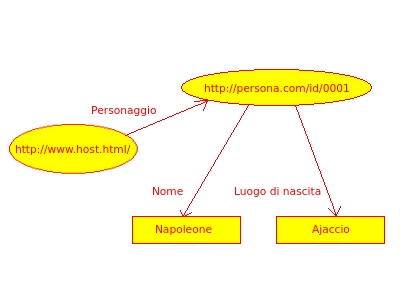
\includegraphics[scale=1]{Napoleone.jpeg}
	\caption{Esempio di Grafo.}
	\label{fig:3}
\end{figure}

che si traduce nel linguaggio rdf:
\begin{lstlisting}[language=XML, basicstyle=\large]
<rdf:Description rdf:about="http://www.host.html/">
	<s:Personaggio rdf:resource="http://persona.com/id/0001"/>
</rdf:Description>
<rdf:Description rdf:about="http://persona.com/id/0001">
 	<s:Nome>Napoleone</s:Nome>
 	<s:Luogo di Nascita>Ajaccio</s:Luogo di Nascita>
</rdf:Description>

\end{lstlisting}
\newpage
Le risorse, i predicati e i valori però possono assumere qualsiasi forma, le principali forme assunte sono:
\begin{itemize}
	\item \textbf{URI/IRI}: come ad esempio la risorsa Napoleone può essere contenuta, per esempio, su DBpedia;\footnote{ sito internet che offre un progetto aperto e collaborativo per l’estrazione e il riutilizzo di informazioni semi-strutturate dalla Wikipedia in italiano. \url{http://it.dbpedia.org/}}
	\item \textbf{Literals}: sono dei valori costanti, come ad esempio date, numeri o anche stringhe.
\end{itemize}
Un' altra caratteristica importante del modello RDF e che è le risorse possono essere raggruppate per formare un insieme; tale insieme prende il nome di \textbf{Contenitore} e in RDF può essere di tre tipi:
\begin{itemize}
	\item \textbf{Bag}, è una lista non ordinata di Risorse e Literals;
	\item \textbf{Sequence}, a differenza di Bag, l'insieme è ordinato;
	\item \textbf{Alternative}, è una lista di risorse che definiscono. un'alternativa per il valore singolo di una proprietà\footnote{Fonte Wikipedia.}
\end{itemize} 
Per rappresentare semanticamente il modello RDF, si utilizza un'estensione chiamata RDF Schema, che fornisce meccanismi per gruppi di risorse correlate e descrive le risorse con le classi, proprietà e valori.\newline Il sistema di classi e delle proprietà di RDF Schema è simile al linguaggio Java e fornisce elementi di base per la descrizione delle ontologie, per vincolare domini e codomini delle relazioni, definire classi di oggetti e relazioni tra classi.
Nelle seguenti tabelle viene descritto le classi e le proprietà utilizzate dal RDF Schema:	\newline		
\begin{table}[!htb]
\begin{center}				
\begin{tabular}{|>{\small}l|>{\small}l|}
	\hline
	\textbf{Nome Classe} & \textbf{Commento}\\				
	\hline 	rdfs:Resource & The class of literal values, e.g. textual strings and integers.\\	
	\hline rdfs:Literal & 	The class of language-tagged string literal values.\\ 			\hline rdf:langString & La classe  language-tagged string literal values.\\			\hline rdf:HTML &	The class of HTML literal values.\\
	\hline rdf:XMLLiteral	& The class of XML literal values.\\
	\hline rdfs:Class & The class of classes.\\
	\hline rdf:Property & The class of RDF properties.\\
	\hline rdfs:Datatype &	The class of RDF datatypes.\\
	\hline rdf:Statement & The class of RDF statements.\\
	\hline rdf:Bag	& The class of unordered containers.\\
	\hline rdf:Seq	& The class of ordered containers.\\
	\hline rdf:Alt	& The class of containers of alternatives.\\
	\hline rdfs:Container & The class of RDF containers.\\
	\hline rdfs:ContainerMembershipProperty & The class of container membership properties.\\
	\hline rdf:List &	The class of RDF Lists.\\
	\hline			
\end{tabular}	
\caption{Tabella delle classi dell'RDF Schema.}	
\end{center}	
\end{table}
\begin{table}[!htbp]
\begin{center}			
\begin{tabular}{|>{\small}l|>{\small}l|>{\small}l|>{\small}l|}
	\hline \textbf{Property name} & \textbf{comment}	& \textbf{domain} & \textbf{range}\\
	\hline rdf:type & The subject is an instance of a class. & rdfs:Resource &	rdfs:Class\\
	\hline rdfs:subClassOf	& The subject is a subclass of a class. & rdfs:Class &	rdfs:Class\\
	\hline rdfs:subPropertyOf	& The subject is a subproperty of a property.&	rdf:Property & rdf:Property\\
	\hline rdfs:domain & A domain of the subject property.& rdf:Property &	rdfs:Class\\
	\hline rdfs:range & A range of the subject property.&	rdf:Property&rdfs:Class\\
	\hline rdfs:label & A human-readable name for the subject. &	rdfs:Resource &	rdfs:Literal\\
	\hline rdfs:comment& A description of the subject resource.& rdfs:Resource &	rdfs:Literal\\
	\hline rdfs:member & A member of the subject resource. &	rdfs:Resource &	rdfs:Resource\\
	\hline rdf:first & The first item in the subject RDF list. & rdf:List&	rdfs:Resource\\
	\hline rdf:rest & The rest of the subject RDF list after the first item. & rdf:List & rdf:List\\
	\hline rdfs:seeAlso & Further information about the subject resource. & rdfs:Resource & rdfs:Resource\\
	\hline rdfs:isDefinedBy & The definition of the subject resource.	& rdfs:Resource & rdfs:Resource\\
	\hline rdf:value &	Idiomatic property used for structured values.&	rdfs:Resource &	rdfs:Resource.\\
	\hline rdf:subject	& The subject of the subject RDF statement. &	rdf:Statement &	rdfs:Resource\\
	\hline rdf:predicate &	The predicate of the subject RDF statement. &	rdf:Statement &	rdfs:Resource\\
	\hline rdf:object & The object of the subject RDF statement.&	rdf:Statement &	rdfs:Resource\\
	\hline		
\end{tabular}
\caption{Tabella delle proprietà dell'RDF Schema.}	
\end{center}	
\end{table}

\newpage

\subsection{Logiche descrittive}
\label{sec:2.2}

La logica descrittiva\footnote{Description Logics} è una notazione formale utilizzata nella rappresentazione della conoscenza. Ogni nodo, oggetto o categoria, è caratterizzato da un elenco di proprietà.
Dato un particolare dominio di conoscenza, la logica descrittiva individua i concetti primari, le categorie più rilevanti, e successivamente analizza le proprietà degli oggetti, al fine di migliorare la descrizione delle classificazioni e delle sotto-classificazioni del dominio di conoscenza. Ogni DL è basata da blocchi sintattici di base che sono:
\begin{itemize}
\item \textbf{Concetti}: corrispondenti a predicati unari che con i quali, combinati tra loro, danno origine a predicati complessi; 
\item \textbf{Ruoli}: corrispondenti a predicati binari ed eventualmente operatori;
\item \textbf{Individui}: costanti usati solo nelle asserzioni.
\end{itemize}
Una base di conoscenza per le DL è costituito da:
\begin{itemize}
\item un insieme finito di assiomi \textbf{Tbox}(terminalogical box);
\item un insieme finito di asserzioni \textbf{Abox} (assertional box).
\end{itemize}

Il TBox contiene frasi che descrivono gerarchie di concetti o di ruoli, mentre l'Abox è un insieme finito di asserzioni di concetto o di ruolo (ad esempio, le relazioni tra gli individui e concetti).
Introduciamo adesso un concetto sintattico molto importante per lo sviluppo delle logiche descrittive, cioè il \textbf{linguaggio descrittivo}.
Un linguaggio descrittivo è il linguaggio attraverso cui si esprimono prescrizioni, aventi la funzione di indirizzare il comportamento degli individui. \newline
\textbf{Definizione}. \newline Un linguaggio descrittivo consiste di una terna di insiemi finiti. \textbf{(C, R, Ob)}. Gli elementi di \textbf{C} sono indicati con le lettere A, B, . . . e sono chiamati concetti atomici; gli elementi di \textbf{R} sono indicati con le lettere R, S, . . . e sono detti
ruoli, mentre gli elementi di \textbf{Ob} sono indicati con le lettere a, b, . . . e sono detti nomi degli oggetti.\footnote{ \url{http://homes.di.unimi.it/~ghilardi/logica2/DL.pdf}). Introduzione alle Logiche Descrittive di Silvio Ghilardi}\newpage Fra i costruttori di concetti annoveriamo certamente gli operatori booleani che indichiamo con $\neg$(negazione), $\sqcap$(intersezione), $\sqcup$(unione). \newline Ci riserveremo anche di usare rispettivamente per il concetto universale $\top$(sempre soddisfatto) e  per il concetto contraddittorio $\bot$(mai soddisfatto).\newline
Un linguaggio descrittivo si può scrivere nel seguente modo $\I = (\Delta^\I,\cdot^\I)$ dove $\Delta^\I$ rappresenta il dominio dell'interpretazione, 
mentre $\cdot^\I$ rappresenta la funzione di interpretazione, che assegna:
\begin{itemize}
	\item ad ogni concetto atomico A$\in$\textbf{C} un insieme  $A^{\I}\subseteq \Delta^\I$;
	\item ad ogni ruolo R$\in$\textbf{R} R una relazione binaria $R^{\I}\subseteq 	\Delta^{\I}$ x $\Delta^{\I} $;
	\item ad ogni nome di oggetto a$\in$\textbf{Ob} un elemento $a^{\I}\in \Delta^\I$.
\end{itemize}  Una volta fatta la premessa sul linguaggio descrittivo, definiamo adesso la logica descrittiva di base chiamata $\alc$\footnote{Attribute Language with Complement} e definiamo i seguenti concetti:
\begin{itemize}
\item $\top^{\I}=\Delta^\I$;
\item $\bot^{\I}=0$;
\item $(C \sqcup  D)^{\I}=C^{\I} \cup D^{\I}$;
\item $(C \sqcap  D)^{\I}=C^{\I} \cap D^{\I}$;
\item $(\neg C)^{\I}=\Delta^{\I} \setminus C^{\I}$;
\item $(\forall R.C)^{\I}=\{a \in \Delta^{I} | (\forall[a,b] \in R^{\I}) (b \in C^{I})\}$;
\item $(\exists R.C)^{\I}=\{a \in \Delta^{I} | (\exists[a,b] \in R^{\I})\wedge (b \in C^{I})\}$.
\end{itemize} La logica descrittiva $\alc$ si può estendere per creare logiche più complesse e articolate; tra i vari costrutti importanti abbiamo:
\begin{enumerate}
\item $\N$: si introducono i costruttori $\geq nR$, $\leq nR$, detti restrizioni numeriche, dove n$\in$N, che sono interpretati come segue:
\begin{center}
		$(\geq nR)^{\I}=\{a \in \Delta^{I}|\#\{b \in \Delta^{I} |[a,b] \in R^{\I}\}\geq n\}$\newline$(\leq nR)^{\I}=\{a \in \Delta^{I}|\#\{b \in \Delta^{I} |[a,b] \in R^{\I}\}\leq n\}$\newline
\end{center} dove $\#\{...\}$ si indica la cardinalità dell'insieme $\{...\}$
\item $\Q$: si introducono i costruttori$\geq nR.C$, $\leq nR.C$, detti restrizioni qualificate
\begin{center}
$(\geq nR.C)^{\I}=\{a \in \Delta^{I}|\#\{b \in C^{I} |[a,b] \in R^{\I}\}\geq n\}$ $(\leq nR.C)^{\I}=\{a \in \Delta^{I}|\#\{b \in C^{I} |[a,b] \in R^{\I}\}\leq n\}$
\end{center}
\item $\Onom$: si introducono gli insiemi finiti di elementi 
detti nominals ($\{a\} o \{a_1,...a_n\} $) interpretati come segue:
\begin{center}
$\{a\}^{\I}=\{a^{\I}\}$
\end{center}
\begin{center}
$\{a_1,...a_n\}^{\I}=\{a_1^{\I},...a_n^{I}\}$
\end{center}
\end{enumerate}\newpage Per estendere il linguaggio si dice che $\I$ è modello $\models$ di:\newline
\textbf{TBox} se:
\begin{center}
	$\I \models C \sqsubseteq D$ se e soltanto se $C^{\I} \subseteq D^{\I}$	
\end{center}
\begin{center}
	$\I \models \T$ se e soltanto se $\I \models \Phi \forall \Phi \in \T $
\end{center}
\textbf{ABox} se: 
\begin{center}
	$\I \models a:C$ se e soltanto se $ a^{\I} \in C^{\I}$
\end{center} 
\begin{center}
	$\I \models (a,b):R$ se e soltanto se $ (a^{\I},b^{\I}) \in R^{\I}$
\end{center}
\begin{center}
	$\I \models \A$ se e soltanto se $\I \models \phi \forall \phi \in \A $
\end{center}
Infine si definisce \textbf{Base di Conoscenza} $\K$ la coppia ordinata $(\A,\T) $ e l'interpretazione $\I$ è modello della base di conoscenza se:
\begin{center}
	$\I \models \K$ se e soltanto se $\I \models \T$ e $\I \models \A $
\end{center}

\newpage

\section{Mappe on-line per siti web}
\label{sec:3}
La realizzazione del portale è stata resa possibile grazie alle librerie fornite dal sito web \textbf{Leaflet}, accessibile digitando l'indirizzo url \url{http://leafletjs.com/}.\newline Leaflet è una moderna libreria open-source realizzata in JavaScript e ha lo scopo di rendere interattive le mappe per utilizzarle in qualsiasi piattaforma si voglia, che sia desktop o mobile. Lo sviluppatore di tale libreria è Vladimir Agafonkin che, con l'aiuto di un team di collaboratori dedicati, ha realizzato una semplice e versatile libreria con soli circa 33 KB di memoria, inoltre utilizzando la tecnologia \textbf{HTML5} e \textbf{CSS3} è accessibile sui browser moderni quali Chrome, Firefox, Safari e Internet Explorer. Può essere anche accessibile per i browser più datati e ha anche una buona e facile documentazione on-line, infine ha un'estesa e vasta gamma di plugin, che si possono facilmente integrare rendendo il più compatto possibile e di facile intuizione.

\subsection{Caricamento mappa}
\label{sec:3.1}
Per preparare il sito web con la mappa interattiva occorre realizzare le seguenti principali procedure:
\begin{itemize}
	\item Inserire nel codice HTML nella sezione \textbf{head} il riferimento al file \textbf{"`leaflet.css"`}
	\item Includere il file scritto in JavaScript \textbf{"`leaflet.js"'}
	\item Inserire un elemento div che ha come parametro \textbf{"`id=map"'} nella sezione \textbf{body}
	\item Settare attraverso la tecnologia CSS3 le caratteristiche della mappa attraverso l'id "`map"'.				
\end{itemize}
Come mostrato nel seguente esempio:
\begin{lstlisting}[language=HTML, basicstyle=\small]
<head>
 <meta charset=utf-8 />
 <title>MAPPA</title>
 <link rel="stylesheet" href="./css/leaflet.css"/>
 <link rel="stylesheet" href="./css/menu.css"/>		
 <script src="./js/leaflet.js"></script>
 <script src="./js/client.js"></script>		
</head>
<body>		
 <div id='map'>
 <div id="loading"><p class="loading">Loading...<p></div>
 </div>					
 <div id="navigation"></div>		
 <script type="text/javascript">
  launch();
 </script>
</body>
\end{lstlisting}
Il secondo passaggio è quello di creare una mappa interattiva, per farlo occorre collegarsi al sito \textbf{\url{www.mapbox.com}}, che fornisce un portale gratuito per creare o modificare una mappa secondo le caratteristiche che si vogliono.
Per fare questo occorre registrarsi al sito web fornendo:
\begin{itemize}
	\item Username;
	\item Cognome;
	\item Nome;
	\item Email;
	\item Password.
\end{itemize}
Una volta effettuato l'accesso bisogna cliccare sul pulsante \textbf{Studio}, situato in alto a destra, poi sul pannello \textbf{Styles} e, infine su \textbf{Create a Style} in questo modo creerà una nuova mappa da poter modellare a seconda delle proprie necessità. Mostrato in Figura \ref{fig:4} e Figura \ref{fig:5}.
\begin{figure}[htpb]
	\centering
	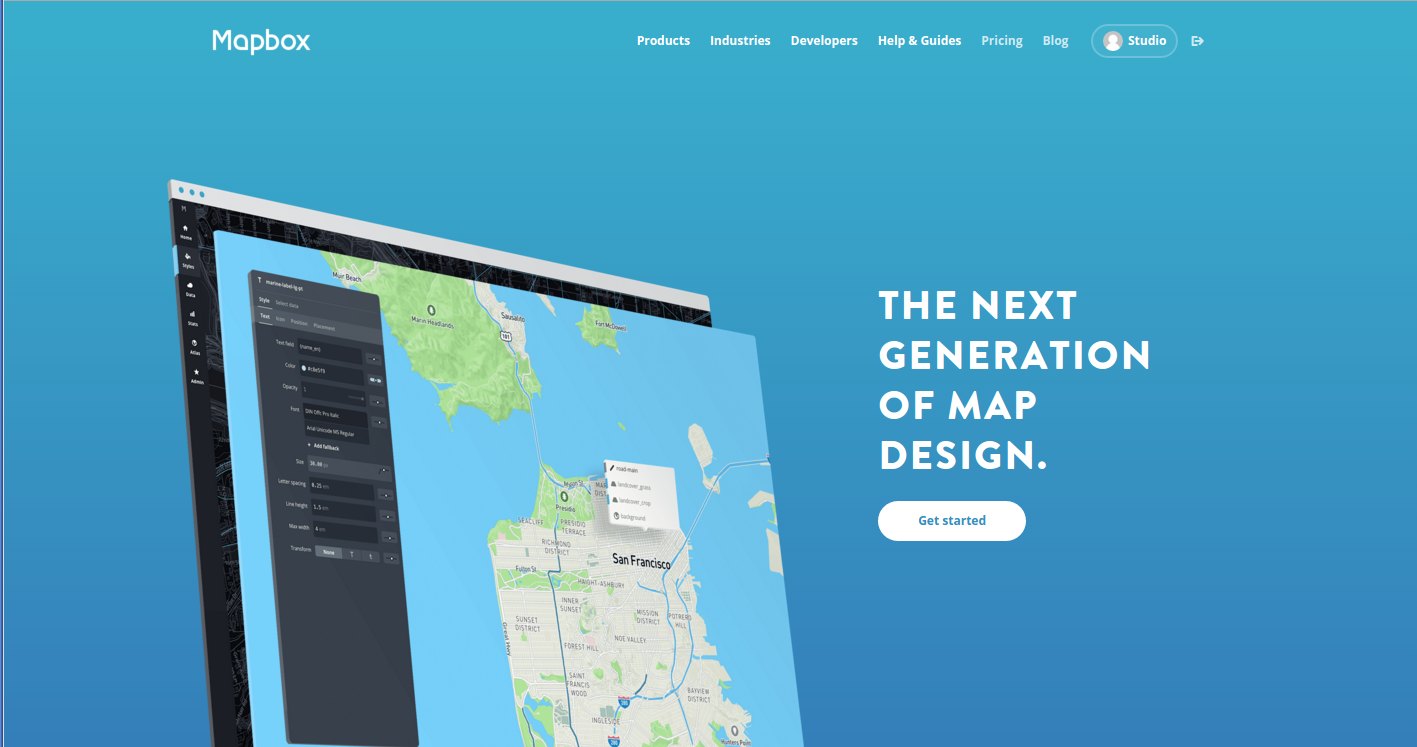
\includegraphics[scale=0.26]{Mapbox.png}
	\caption{Sito di Mapbox.}
	\label{fig:4}
\end{figure}
\begin{figure}[htpb]
	\centering
	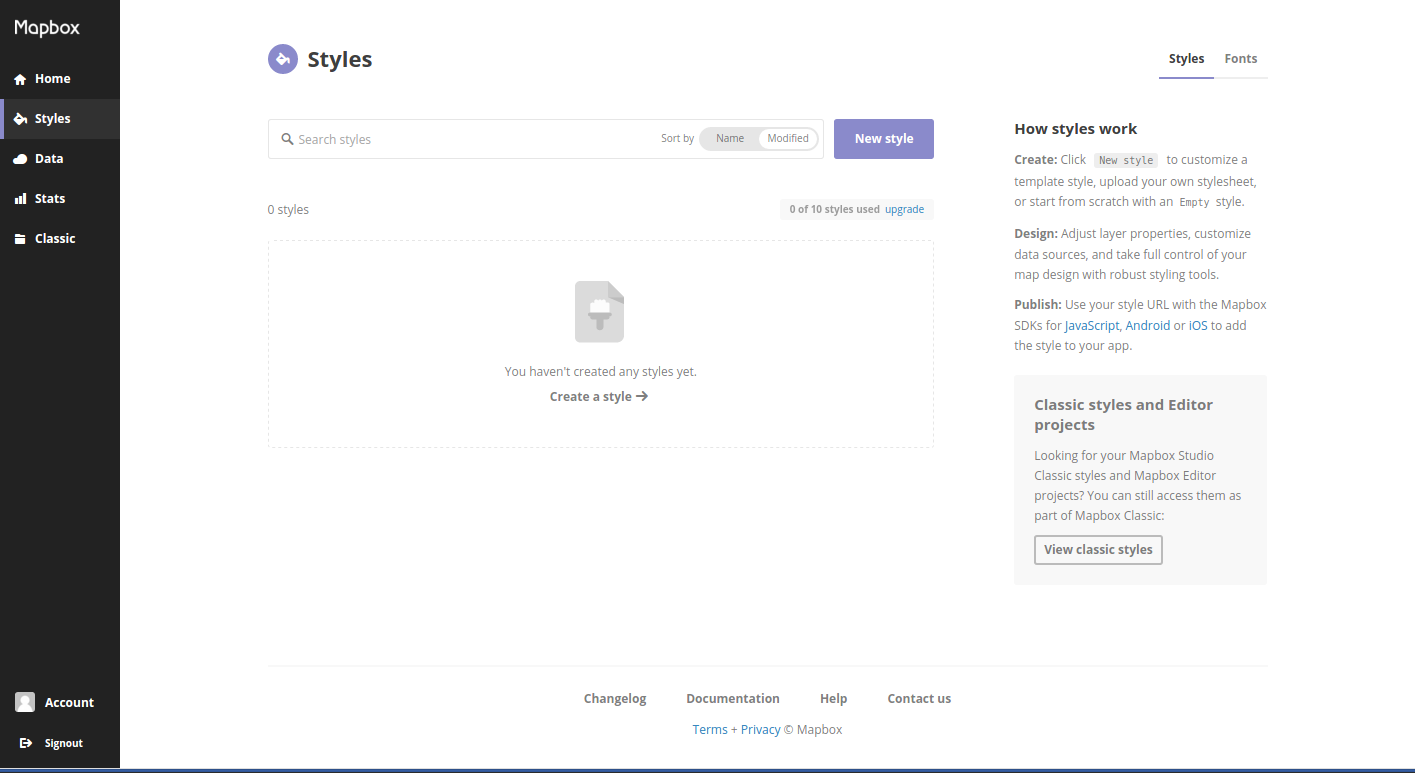
\includegraphics[scale=0.26]{Styles.png}
	\caption{Pannello Styles.}
	\label{fig:5}
\end{figure}\newline
Una volta creata la mappa, cliccare sul pannello \textbf{Edit}, in questo modo si aprirà una nuova pagina.
Sul pannello  a sinistra è indicata la consolle per modellare la mappa, possiamo scegliere i colori delle strade, dell'acqua, della terra e pianure e dello sfondo.\newline
Sul pannello di destra, invece, è indicato lo zoom e le coordinate, cioè la latitudine e la longitudine. Sistemate tutte le modifiche per confermare il progetto della mappa cliccare sul pulsante \textbf{Publish}.
Cliccando sul nome della mappa, nel pannello \textbf{Styles}, a destra è indicato l'indirizzo url per poter pubblicare la mappa.
\newline
In Figura \ref{fig:6} è mostrato la schermata \textbf{Edit}.
\begin{figure}[ht]
	\centering
	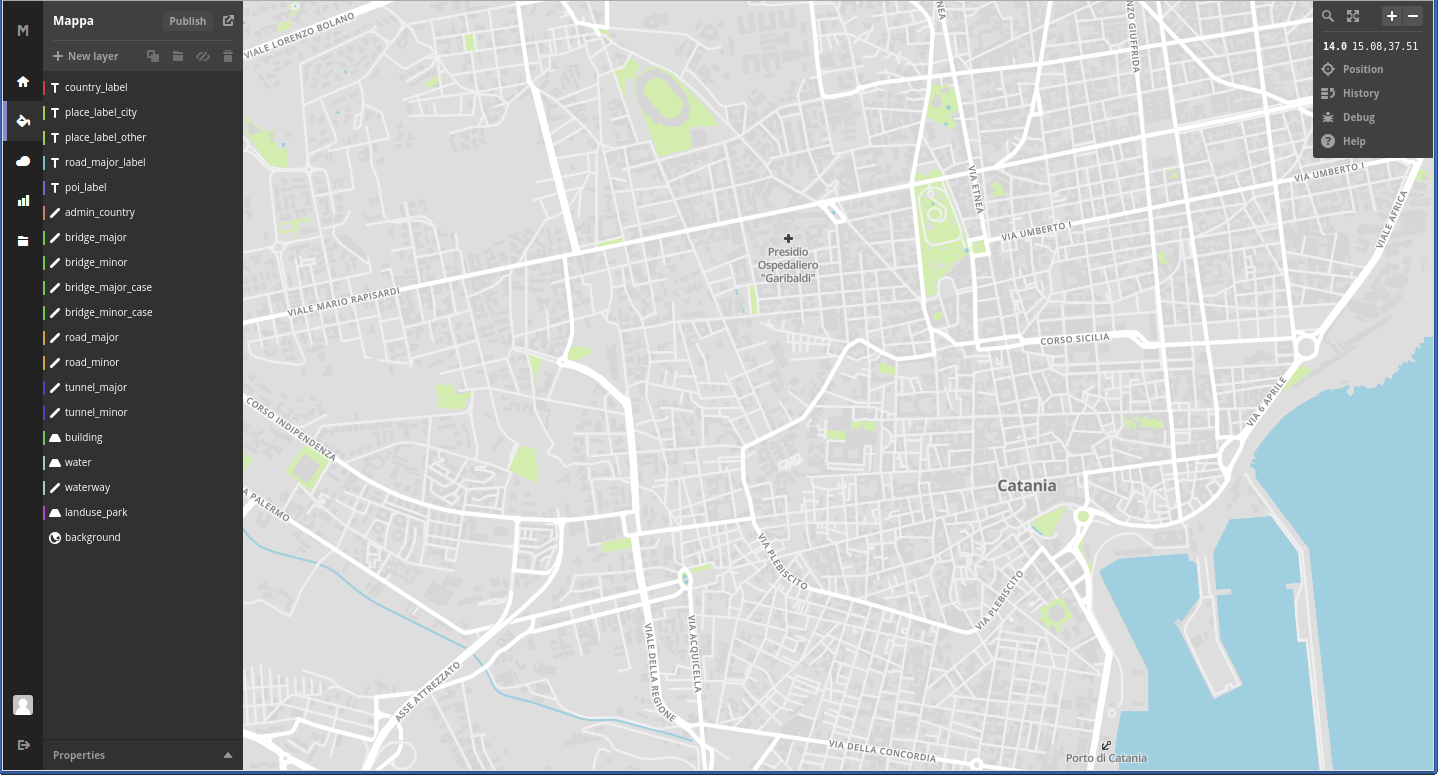
\includegraphics[scale=0.26]{Edit.png}
	\caption{Pannello Edit.}
	\label{fig:6}
\end{figure}\newpage		
Per inserire la mappa sul codice sorgente e caricarla nella pagina web, bisogna inizializzarla fornendo le coordinate geografiche della posizione e il livello dello zoom. Tali informazioni sono reperibile sul pannello Edit come mostrato in  Figura \ref{fig:7}, e devono essere inserite nella sezione body della file \textbf{index.html}.
\begin{figure}[htbp]
	\centering
	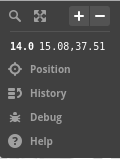
\includegraphics[scale=1]{coordinate.png}
	\caption{Coordinate e zoom mappa.}
	\label{fig:7}
\end{figure}\newline

Il codice da inserire e da mettere nella sezione body ed è il seguente:

\begin{lstlisting}[language=HTML, basicstyle=\large]
<body>		
<div id=`map'>
<script type="text/javascript">
 var auxmap = L.map(`map').setView([37.51, 15.08], 14);
</script>
</div>
</body>
\end{lstlisting}
				
Dalla codice si evince che all'interno delle parentesi, sono inserite le coordinate geografiche presenti nella Figura \ref{fig:7}, inoltre lo script utilizzato è sempre JavaScript.
Il prossimo passaggio è quello di inserire la mappa utilizzando il comando \textbf{tileLayer}. Tale comando permette di inserire la mappa creata sul sito di Mapbox, definendo lo zoom massimo possibile, gli attributi, l'identificativo della mappa e l'access token. Di seguito abbiamo il codice sorgente:
\begin{figure}[htb]
\begin{lstlisting}[language=HTML, basicstyle=\large]
<body>		
<div id=`map'>
<script type="text/javascript">
 var auxmap = L.map(`map').setView([37.51, 15.08], 14);
 L.tileLayer(`https://api.tiles.mapbox.com/v4/{id}/{z}/{x}/{y}.png?'+ 
  `access_token={pk.eyJ1IjoiYW5kcmVhY29zdGF6emEiLCJhIjoiN3VXTWIxayJ9.'+
  `iG0HHcB2nWD2-I9-tx0vhA}', {
 maxZoom: 18,
 attribution: `Map data &copy; 
 <a href="http://openstreetmap.org">OpenStreetMap</a> contributors, '+
  `<a href="http://creativecommons.org/licenses/by-sa/2.0/">CC-BY-SA</a>, '+
  `Imagery c <a href="http://mapbox.com">Mapbox</a>',
 id: `mapbox://styles/andreacostazza/cijyrg3yt00zsbpm3orpxkj2l'
 accessToken: `pk.eyJ1IjoiYW5kcmVhY29zdGF6emEiLCJhIjoiN3VXTWIxayJ9.'+
 `iG0HHcB2nWD2-I9-tx0vhA'
	}).addTo(map);
</script>
</div>
</body>
\end{lstlisting}
\end{figure}
\newpage
Sul codice precedente per il caricamento della mappa, si nota che nella prima voce è indicato il collegamento ipertestuale della mappa, alla voce \textbf{attribution} sono indicate le licenze, mentre alla voce \textbf{id}, è specificato l'identificativo della nostra mappa, che si ricava dal sito Mapbox alla sezione \textbf{Styles} come mostrato in Figura \ref{fig:5} accanto alla voce Edit.
Infine alla voce \textbf{accessToken}, si deve indicate quel valore disponibile, sempre nel pannello \textbf{Styles}, a destra. \newline
Seguendo le procedure appena indicate, la mappa verrà visualizzata correttamente nella nostra pagina web.

\subsection{Creazione delle icone, dei markers e dei popups}
\label{sec:3.2}
Attraverso il metodo \textbf{L.Icon} è possibile creare un icona che identifica un determinato punto della mappa. Per prima cosa occorre scegliere un'immagine, dopodiché attraverso \textbf{iconUrl} è possibile caricarla specificando il percorso del file; se si dispone anche di un immagine con l'ombra bisogna caricarla con \textbf{shadowUrl} sempre specificando il percorso del file. Poi bisogna specificare la grandezza dell'icona e dell'ombra, attraverso i parametri \textbf{iconSize} e \textbf{shadowSize} come è evidenziato nel codice seguente. Infine caricare il marker attraverso il metodo \textbf{L.marker}, dove vengono specificate le coordinate.
\begin{figure}[htb]
\begin{lstlisting}[language=HTML, basicstyle=\large]
<body>		
<div id='map'>
<script type="text/javascript">
var map=L.map('map')setView([37.583,14.071],9);
L.tileLayer('https://{s}.tiles.mapbox.com/v3/{id}/{z}/{x}/{y}.png',{
        maxZoom: 18,
        attribution: 'Map data &copy; 
  <a href="http://openstreetmap.org">OpenStreetMap</a> contributors,'+
 '<a href="http://creativecommons.org/licenses/by-sa/2.0/">CC-BY-SA</a>,'+
	'Imagery c <a href="http://mapbox.com">Mapbox</a>',
	id: 'andreacostazza.ik9ap86i'
	}).addTo(map);
var iconBlue= L.icon({
	iconUrl: './icon/marker-icon.png',
	shadowUrl: './icon/marker-shadow.png',
			
	iconSize: [25,41],
	shadowSize: [41,41],
	iconAnchor:[lat,lon],
	shadowAnchor:[lat,lon],
	popupAnchor:[-25,-10]
	});
	
	var marker = L.marker([lat, lon],{icon:iconBlue});		
	marker.addTo(map);
</script>
</div>
</body>
\end{lstlisting}
\end{figure}
\newpage
\section{SPARQL}
\label{sec:4}
Il linguaggio \textbf{SPARQL}\footnote{SPARQL Protocol and RDF Query Language} è un linguaggio di interrogazione per dati rappresentati tramite il \textbf{Resource Description Framework (RDF)}.
SPARQL è un elemento essenziale per lo sviluppo del web semantico e consente di estrarre informazioni in tutto il mondo.\newline 
La struttura del database è un insieme di triple "soggetto-predicato-oggetto", però a differenza dell'RDF, le triple possono essere delle variabili, che sono indicate con il punto interrogativo ?, oppure costanti.

\begin{center}	
	\textbf{?title rdf:label ?name}
\end{center}

Nell'esempio proposto il soggetto e l'oggetto sono delle variabili, mentre il predicato è una costante che fa riferimento a rdf.\footnote{rdf:\url{http://www.w3.org/TR/rdf-schema/}}\newline
I dati ottenuti, facendo una query\footnote{Interrogazione} allo SPARQL, è una tabella molto simile a quelle utilizzate nei database relazionali in SQL; si tratta di una tabella dove le colonne sono composte dal risultato del soggetto, del predicato e dell'oggetto. 

\subsection{Il modello Turtle}
\label{sec:4.1}
La sintassi utilizzata nello SPARQL è simile a Turtle\footnote{Terse RDF Triple Language} per esprimere modelli di query. \newline 
Il Turtle è anch'esso un formato per esprimere i dati nel \textbf{Resource Description Framework (RDF)},  anche in questo caso le informazioni vengono rappresentate attraverso le triple, ciascuna delle quali è costituito da un soggetto, un predicato, e un oggetto. Ogni elemento è espresso come indirizzo URI/IRI come mostrato in Figura 6.
\begin{figure}[htbp]
	\centering
	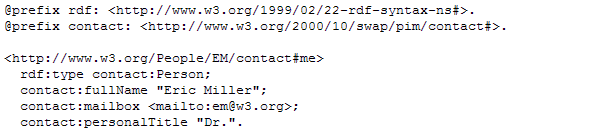
\includegraphics[scale=1]{turtle.png}
	\caption{Esempio Codice Turtle.}
	\label{fig:8}
\end{figure}
Gli indirizzi URI vengono racchiusi tra "<" ed ">" e possono essere abbreviati attraverso il comando \textbf{@prefix}, a cui viene associato un nome che può essere richiamato in diversi parti del file.\newline
Turtle è un'alternativa a RDF/XML, ma a differenza di quest'ultimo, Turtle non si basa su XML ed è più facile da modificare, inoltre risulta molto più leggibile.\newline
Nel 2011, il World Wide Web Consortium (W3C) ha iniziato a lavorare su una versione aggiornata di RDF, ed ha pubblicato la documentazione il 25 febbraio 2014.\footnote{La pubblicazione si trova al sito https://www.w3.org/TR/turtle/}
\newpage
\subsection{Comandi principali}
\label{sec:4.2}
Il linguaggio SPARQL è composto da tre comandi principali:
\begin{itemize}
	\item \textbf{PREFIX:} dichiara prefissi e namespace e, come nel Turtle, per
abbreviare il percorso URI si associa un nome che verrà
richiamato all'interno di WHERE (ad es gr:offers può essere
scritto anche <http://purl.org/goodrelations/v1offers>)
	\item \textbf{SELECT:} identifica le variabili che verranno visualizzate, sotto forma di tabella, dal risultato dell' interrogazione. È spesso
accompagnato da *, che seleziona tutte le variabili di una
interrogazione, e DISTINCT, che esclude dal risultato i valori
duplicati;
	\item \textbf{WHERE:} seleziona il criterio di selezione da applicare ai dati; è composto da un blocco, delimitato dalle parentesi graffe (\{...\}),
dove al suo interno può esserci una o più triple, separati da un
punto fermo.
	\end{itemize}
Come in SQL, anche in SPARQL esiste il comando \textbf{FROM}, contenente un
indirizzo IRI, che identifica tutto il set di dati presenti, dove l'interrogazione dovrà essere svolta; è spesso accompagnato dal comando NAMED usato per specificare più indirizzi IRI.
Inoltre SPARQL fornisce diversi comandi per una maggiore flessibilità sulle
interrogazioni. Nella tabella seguente sono riportate quelle più utilizzate:
\begin{table}[htb]
\begin{center}				
\begin{tabular}{|>{\small}l|>{\small}l|>{\small}l|}
	\hline \textbf{Nome Comando} & \textbf{Cosa fa} & \textbf{Attributi}\\				\hline FILTER: & Filtra i valori visualizzati. & \textbf{regex} si utilizza per espressioni regolari.\\
	\hline OPTIONAL: & Prevede l'assenza di alcuni termini & Le variabili compariranno prive di valore.\\
	\hline ORDER BY: & Ordina il risultato in base ad una variabile specifica. & DESC ordinamento decrescente. \\
	\hline LIMIT: & Limita la visualizzazione. & Accompagnata da valori numerici \\
	\hline a:	& Visualizza le classi a cui appartiene una variabile. & Alternativa a rdf:type\\
	\hline			
\end{tabular}	
\caption{Tabella dei comandi principali di SPARQL.}	
\end{center}	
\end{table}
\newpage
\subsection{Libreria javascript per interrogazioni SPARQL}
\label{sec:4.3}
Per fare un interrogazione in SPARQL, JavaScript ha bisogno di una chiamata AJAX\footnote{Vedi Capitolo \ref{sec:5.2}} e della codifica JSON\footnote{Vedi Capitolo \ref{sec:5.3}}.
Nel progetto sono date rispettivamente dalla variabile \textbf{xmlhttp}, che fa la chiamata AJAX tramite il metodo \textbf{getHTTPObject()} e restituisce il risultato tramite \textbf{responseText}.
La richiesta AJAX, inoltre, utilizza \newline \textbf{setRequestHeader("Accept", "application/sparql-results+json");} \newline in questo modo i risultati ottenuti sono visualizzati secondo la codifica JSON.
Il codice utilizzato nel progetto è il seguente:
\begin{figure}[!htb]
\begin{lstlisting}[language=HTML, basicstyle=\large]
<body>		
<div id='map'>
<script type="text/javascript">
//Created SPARQL query
function createSparqlQuery(endpoint,query,map,callback){	
 var querypart = "query=" + escape(query);
 // Get our HTTP request object.
 var xmlhttp = getHTTPObject(); //Called AJAX
 //Include POST OR GET
 xmlhttp.open('POST', endpoint, true); 
 xmlhttp.setRequestHeader('Content-type',
 	'application/x-www-form-urlencoded');
 xmlhttp.setRequestHeader("Accept", 
  "application/sparql-results+json");	
 xmlhttp.onreadystatechange = function() {
  if(xmlhttp.readyState==4 ){
   if(xmlhttp.status==200){				
	 callback(xmlhttp.responseText,map); //JSON code
	 }else
	// Error
	alert("Error: Status: "+ xmlhttp.status + "Response: "
	+ xmlhttp.responseText);
	}	
 };
 // Send the query to the endpoint.
 xmlhttp.send(querypart);	
}
</script>
</div>
</body>
\end{lstlisting}
\end{figure}\newline
Basta scrivere la query utilizzando la nomenclatura dello SPARQL descritta precedentemente e fornire l'indirizzo URI della base di conoscenza; la variabile utilizzata nel progetto per scrivere la query è \textbf{query}, mentre per far riferimento alla base di conoscenza si utilizza endpoint.
\newpage
\section{Ontologie per la rappresentazione dei servizi pubblici}
\label{sec:5}
L’Agenzia per l’Italia Digitale (AgID\footnote{\url{www.agid.gov.it}}) ha l'obiettivo di pubblicare dati e documenti relativi ai servizi, alla struttura e alle attività svolte sul sito e di fornire a pubbliche amministrazioni, imprese e cittadini le tecniche utilizzate dal Web Semantico. In pratica vengono forniti vocabolari, sviluppati tramite la pubblicazione \textbf{Linked Open Data}. Tale metodo consiste nello strutturare i dati in modo da poter essere interconnessi e diventare più utili attraverso delle interrogazioni, fatte per esempio dallo linguaggio SPARQL. 
Nella tabella successiva vengono indicati alcuni dei principali vocabolari utilizzati.

\begin{table}[!htbp]
\begin{center}				
\begin{tabular}{|>{\small}l|>{\small}l|>{\small}l|}
	\hline	\textbf{Vocabolario} & \textbf{Namespace} & \textbf{URL}\\				
	\hline	Friend Of A Friend & foaf & http://xmlns.com/foaf/spec/.\\
	\hline	Core Location & locn & http://www.w3.org/ns/locn.\\
	\hline	Organization Ontology & org & http://www.w3.org/TR/vocab-org/\\
	\hline			
\end{tabular}	
\caption{Tabella Vocabolari.}	
\end{center}	
\end{table}
Analizzeremo in dettaglio i vocabolari \textbf{Core Location} e \textbf{Organization Ontology}.
Il \textbf{Core Location} è un vocabolario utilizzato per rappresentare qualsiasi luogo in termini di nome, di indirizzo o di coordinate. Tale vocabolario fa parte del progetto \textbf{ISA}.\footnote{Interoperability Solutions for European Public Administrations. \url{http://ec.europa.eu/isa/}}. L'idirizzo URI utilizzato è \url{http://www.w3.org/ns/locn\#} ed usa il prefisso \textbf{locn}. \newline Il vocabolario è composto da tre classi che sono:
\begin{itemize}
	\item \textbf{Location}: utilizzata per identificare luoghi, città, stati,  
	\item \textbf{Address}: utilizzata per gli indirizzi.Questa classe fa riferimento anche ad altre informazioni quali la casella postale, al numero civico, al codice di avviamento postale e così via,
	\item \textbf{Geometry}: fornisce latitudine e longitudine.
\end{itemize} 
\textbf{Organization Ontology}, invece, è utilizzato per modellare le pubbliche amministrazioni, fornendo indicazioni relative ad organizzazioni, membri, macrostrutture e strutture fisiche.
L'indirizzo URI utilizzato è \url{http://www.w3.org/TR/vocab-org/\#} ed usa il prefisso \textbf{org}.\newline
La classe principale è \textbf{Organizzation} che scompone le organizzazioni in strutture gerarchiche.
Mentre la classe \textbf{FormalOrganizzation} scompone un'organizzazione che è riconosciuta in tutto il mondo, come ad esempio i governi.
Per rappresentare un'organizzazione, come ad esempio un dipartimento o unità di supporto, che è parte di una organizzazione più grande si usa la classe \textbf{OrganizationalUnit}.
Organization Ontology estende e utilizza termini da altri vocabolari, riportati nella seguente tabella:
\begin{table}[!htb]
\begin{center}				
\begin{tabular}{|>{\small}l|>{\small}l|}
	\hline \textbf{Prefisso} & \textbf{Namespace}\\				
	\hline foaf & http://xmlns.com/foaf/0.1/\\
	\hline gr & http://purl.org/goodrelations/v1\#\\
	\hline prov & http://www.w3.org/ns/prov\#\\
	\hline owl & http://www.w3.org/2002/07/owl\#\\
	\hline rdf & http://www.w3.org/1999/02/22-rdf-syntax-ns\#\\
	\hline rdfs & http://www.w3.org/2000/01/rdf-schema\#\\			
	\hline time & http://www.w3.org/2006/time\#\\
	\hline skos & http://www.w3.org/2004/02/skos/core\#\\					
	\hline vcard & http://www.w3.org/2006/vcard/ns\#\\											\hline 	dct & http://purl.org/dc/terms/\\			
	\hline
\end{tabular}	
\caption{Tabella degli stati di XMLHttpRequest.}	
\end{center}	
\end{table}\newpage
Tali vocabolari servono per organizzare al meglio la struttura organizzativa di aziende, società e comuni.
Nel progetto è stato utilizzato un vocabolario creato dal \textbf{Dott.Cristiano Longo} che fa riferimento allo macro struttura del Comune di Catania.
Tale vocabolario si trova al seguente sito \url{ttp://dydra.com/cristianolongo/comune-di-catania/sparql}.\newline
Tramite questo endpoint, si fa una specifica interrogazione in SPARQL, attraverso una chiamata AJAX. I dati ottenuti sono codificati tramite la codifica JSON.
\subsection{Menù gerarchici}
\label{sec:5.1}
Un menu gerarchico è una struttura ad albero che simula l'aspetto e il comportamento della struttura a cartelle e sottocartelle utilizzato in tutti i S.O.\footnote{Sistemi Operativi.}. Questo tipo di menù viene utilizzato nella stragrande maggioranza dei siti web proprio perché è facile da implementare e non occupa moltissimo spazio, inoltre in questo modo si possono realizzare strutture annidate e complesse ricche di voci, che sono ideali per l'organizzazione.\newline 
Nel progetto il menù gerarchico è creato dinamicamente, cioè ad ogni valore che viene passato si controlla il genitore e i figli associati.
Per comprendere meglio elenchiamo i metodi e le classi, realizzati in Javascript, per la creazione del menù:
\begin{itemize}
	\item Classe \textbf{Tree}, che implementa l'albero N-ario.\footnote{Albero con n figli} Un albero N-ario ha i due elementi fondamentali che sono la \textbf{radice},\footnote{Root.} che ha n nodi che vengono chiamati figli e le \textbf{foglie},\footnote{Leaf.} che sono i nodi senza figli. Tutti gli altri nodi vengono chiamati nodi interni\footnote{Fonte Wikipedia}.
La classe Tree	ha le seguenti variabili:
\begin{itemize}
	\item \textbf{value}: può essere qualsiasi valore, in questo progetto la si associa ad un indirizzo URI/IRI o a un nome della gerarchia o a una struttura complessa contenete sia URI che nomi;
	\item \textbf{children}: un array,\footnote{Struttura dati complessa composto da celle di lunghezza n.}, contenente i figli di un nodo.
\end{itemize}
ed i seguenti metodi
\begin{itemize}
	\item \textbf{addChild(value)}: aggiunge ad un nodo un figlo;
	\item \textbf{getChild()}: stampa a video di tutti i figli di un nodo;
	\item \text{preOrder(), postOrder()}: metodi utilizzati per la visita dell'albero;
	\item \textbf{high(), frontier()}: metodi informativi dell'albero.
\end{itemize}			
	\item Classe \textbf{Description}, struttura dati complessa che contiene tre variabili che sono:
\begin{itemize}
	\item \textbf{uri}: Indirizzo IRI/URI di un valore;
	\item \textbf{name}: Nome di un valore;
	\item \textbf{homepage}: Indirizzi IRI/URI che si collega alla pagina principale del sito web.
\end{itemize}	
i metodi di tale classe sono:
\begin{itemize}
	\item \textbf{getUri()}: Restituisce il valore di uri;
	\item \textbf{getName()}: Restituisce il valore di name;
	\item \textbf{getHomepage()} Restituisce il valore di homepage.
\end{itemize} \newpage
\item Classe \textbf{Storage}, che è un contenitore di tutti i nodi, compresa la radice con i seguenti metodi:
\begin{itemize}
	\item \textbf{add(Description)}: istanza classe Tree(crea nodo all'interno dello storage);
	\item \textbf{get(Uri)}: restituisce nodo con la URI, se esiste; altrimenti NULL;
	\item \textbf{getTrees()}: restituisce tutte le foglie.
\end{itemize}
\end{itemize}	
Il menù gerarchico nel progetto è creato sfruttando le classi appena elencate, in più è arricchito con due metodi che sono:
\begin{itemize}
	\item \textbf{createLiMenu()}, che crea un lista utilizzando i tag:
	\begin{itemize}
		\item <ul> definisce una lista non ordinata;
		\item <li> creare la liste non ordinate, è sempre associato al tag <ul>.
	\end{itemize}
	\item \textbf{createMenu()}, che crea il menu dinamico.
\end{itemize}
Di seguito viene specificato, attraverso lo pseudo-codice, la creazione di tale menu:\newline
\textbf{Pseudo codice}
	\begin{itemize}
	\item Attraverso la chiamata AJAX e la codifica JSON otteniamo i dati dalla base di conoscenza;
	\item Vengono create le variabili parent e child;
	\item A parent viene associato il nodo, mentre a child il figlio;
	\item Per ogni coppia di parent e child:
		\begin{itemize}
		\item ricerca di parent all'interno di Storage; 
		\item se lo trova va avanti, altrimenti lo crea(metodo add di Storage);
		\item ricerca di child all'interno di Storage;
		\item se lo trova va avanti, altrimenti lo crea(metodo add di Storage);
		\item associa child a parent;
		
		\end{itemize}		
	\item restituisce l'albero dallo Storage;
	\item crea il menu attraverso il metodo createLiMenu.
	\end{itemize} 	
Il risultato sarà il seguente menù:
\begin{figure}[htpb]
	\centering
	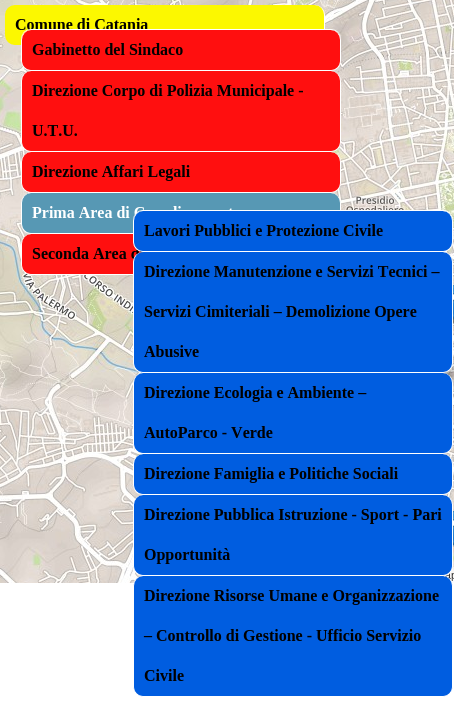
\includegraphics[scale=0.4]{menu.png}
	\caption{Il menù gerarchico del progetto.}
	\label{fig:9}
\end{figure}
\subsection{Codifica JSON}
\label{sec:5.2}
La codifica JSON\footnote{JAVASCRIPT Object Notatio} è un formato convenzionale che serve per lo scambio di dati fra client e server. Ha la stessa nomenclatura dell'XML, ma  a differenza di quest'ultimo, è molto leggero da analizzare, ed è anche molto semplice da realizzare.
Il JSON è scritto interamente in JavaScript ed è  utilizzato, principalmente, per le chiamate AJAX.\footnote{Vedi Paragrafo \ref{sec:5.3}}. I dati della codifica JSON possono essere di qualunque tipo. I principali valori sono:
\begin{itemize}
	\item boolean;
	\item stringhe;
	\item interi; 
	\item array sia semplici che associativi;
	\item null;
\end{itemize} 
Quindi tale codifica può essere utilizzata in un qualsiasi linguaggio di programmazione.
Inoltre è facilmente leggibile da quasi tutti i browser moderni, visto che hanno il supporto nativo a JSON, mentre per quelli sprovvisti occorre utilizzare il comando \textbf{eval}. \newline Di seguito vediamo un esempio di codifica JSON
	\begin{figure}[htb]
		\centering
		\begin{lstlisting}[language=HTML, basicstyle=\large]
{
  "uri": "www.example.com",
  "name": "Example",
  "comment": "A example page",
  "group": [
    {
      "firstUri": "www.example1.com",
      "firstValue": "Example1",
      "firstComment": "First example page"       
    },   
    {
      "second_uri": "www.example2.com",
      "second_value": "Example2" ,
      "second_comment": "Second example page"
    }
  ]
}
		\end{lstlisting}
 \end{figure}\newline
Ogni dato ha la forma coppia ``nome'' : ``valore'', ed è separato dall'altro tramite la virgola e, inoltre sia i nomi che i valori sono racchiusi tra doppie virgolette.\newline
Le parentesi graffe contengono oggetti: \newline \{``firstUri'': ``www.example1.com'',``firstValue'': ``Example1'',\newline ``firstComment'':``First example page''   \} \newline
Le parentesi quadre contengono array: \newline ``group'': [\{``firstUri'':``www.example1.com'',``firstValue'': ``Example1'',\newline ``firstComment'': ``First example page''\},\newline\{``secondUri'': ``www.example2.com'',``secondValue'': ``Example2'', \newline ``secondComment'': ``Second example page''\}]
\newpage
\subsection{Chiamata AJAX}
\label{sec:5.3}
Il metodo AJAX\footnote{Asynchronous JAVASCRIPT and XML} è stato creato da Jesse Garrett ed è un modo di riutilizzare gli standard internet esistenti. 
Attraverso il linguaggio di Javascript, che si interfaccia con XML, un \textbf{client}\footnote{Indica una componente che accede ai servizi o alle risorse di un'altra componente detta server. Fonte Wikipedia} richiama le informazioni in modo veloce e trasparente, cioè in maniera asincrona. Per effettuare una chiamata AJAX abbiamo bisogno di un oggetto specifico chiamato \textbf{XMLHttpRequest} che serve per lo scambio di dati in modo asincrono con un server.
Tale oggetto viene utilizzato nel progetto dal metodo \textbf{getHTTPObject()}
di cui riportiamo il codice:
\begin{figure}[htb]
\begin{lstlisting}[language=HTML, basicstyle=\large]
function getHTTPObject(){
var xmlhttp;
if(!xmlhttp && typeof XMLHttpRequest != 'undefined'){
 try{
  // Code for old browser
  xmlhttp=new ActiveXObject('Msxml2.XMLHTTP');
 }
 catch(err){
  try{
   // Code for IE6, IE5
   xmlhttp=new ActiveXObject("Microsoft.XMLHTTP");
  }
  catch(err2){
   try{
	 // Code for IE7+, Firefox, Chrome, Opera, Safari
	 xmlhttp=new XMLHttpRequest();
   }
   catch(err3){
    xmlhttp=false
   }
  }			
 }
}
 return xmlhttp;
}		
\end{lstlisting}
\end{figure}\newline
Ogni Browser web ha la sua richiesta, nel caso di Browser datati, come IE,\footnote{Internet Explorer} l'oggetto XMLHttpRequest, viene restituito da \textbf{ActiveXObject}, mentre i moderni browser tale oggetto è supportato nativamente.\newpage Per inviare una richiesta ad un server, bisogna utilizzare il seguente codice:
\begin{figure}[htb]
\begin{lstlisting}[language=HTML, basicstyle=\large]
var xmlhttp = getHTTPObject();
//Include POST OR GET
xmlhttp.open('POST', endpoint, true); 
xmlhttp.setRequestHeader('Content-type',
  'application/x-www-form-urlencoded');
xmlhttp.setRequestHeader("Accept", 
  "application/sparql-results+json");	
xmlhttp.onreadystatechange = function() {
 if(xmlhttp.readyState==4 ){
  if(xmlhttp.status==200){				
   callback(xmlhttp.responseText,map);
  }else
  // Error
  alert("Error: Status: "+ xmlhttp.status + "Response: "
		+ xmlhttp.responseText);
 }	
};
// Send the query to the endpoint.
xmlhttp.send(querypart);
\end{lstlisting}
\end{figure}\newline
Una volta creato un oggetto di tipo \textbf{getHTTPObject()}, la variabile \textbf{xmlhttp}, con i metodi \textbf{open} e \textbf{send}, si apre e si invia la richiesta al server.\newline
Con open si posso effettuare due tipi di chiamata. La prima può essere fatta tramite GET, mentre la seconda può essere fatta tramite una chiamata POST. Per una chiamata di tipo POST però bisogna impostare gli headers,\footnote{serie di coppie chiave/valore specifici per uno scambio dati via interne} dato dal comando:
\begin{figure}[htb]
\begin{lstlisting}[language=HTML, basicstyle=\large]
xmlhttp.setRequestHeader('Content-type',
  'application/x-www-form-urlencoded')
\end{lstlisting}
\end{figure}\newline
La variabile \textbf{onreadystatechange} chiama la funzione ogni volta che il valore ottenuto dal metodo readyState cambia.
Il metodo \textbf{readyState} tiene traccia dello stato di XMLHttpRequest e può assumere determinati valori:
\begin{table}[htb]
\begin{center}				
\begin{tabular}{|>{\small}l|>{\small}l|}
	\hline	\textbf{Valore} & \textbf{Commento}\\				
	\hline	0 & richiesta non inizializzata.\\
	\hline	1 & connessione server stabilita.\\
	\hline	2 & richiesta ricevuta.\\
	\hline	3 & richiesta in processo.\\
	\hline	4 & richiesta finita e responso è pronto.\\
	\hline			
\end{tabular}	
\caption{Tabella degli stati di XMLHttpRequest.}	
\end{center}	
\end{table}\newpage
Infine con il metodo \textbf{status} si controlla la risposta dal server e può  assumere diversi valori:
\begin{itemize}
	\item 200 Il server è stato trovato;
	\item 403 Forbidden;
	\item 404 Server Not Found;
	\item 500 Internal Server Error;
	\item ...
\end{itemize}
Quando si verifica che \textbf{readyState} ha valore 4 e \textbf{status} ha valore 200, il client comunica con il server e il risultato, dato dal metodo \textbf{responseText} viene convertito in una stringa che poi, successivamente,  si applicherà la codifica JSON.
Tuttavia però tale chiamata non sempre va a buon fine. I browser moderni hanno una sorta di restrizione\footnote{Same-domain-policy}, cioè che non si può fare una richiesta HTTP da risorse che si trovano su server diversi rispetto a quello iniziale che ha inviato lo script.\newline
Tale richiesta viene chiamata richiesta \textbf{Cross-domain}, che verrà affrontata nel Capitolo \ref{sec:6.4}.
\newpage
\section{Presentazione e codice dell'applicazione}
\label{sec:6}
\subsection{Programmi utilizzati}
\label{sec:6.1}
\subsection{HTML}
\label{sec:6.2}
\subsection{Css}
\label{sec:6.3}
\subsection{Il problema delle richieste Cross-Domain}
\label{sec:6.4}


\end{document}


